%! suppress = EscapeHashOutsideCommand
%! suppress = TooLargeSection
%! suppress = MissingLabel

% * Make friends tikz & colors
%   https://en.wikibooks.org/wiki/LaTeX/Colors
% * To enable vertical top alignment globally
%   https://tex.stackexchange.com/questions/9889/positioning-content-at-the-top-of-a-beamer-slide-by-default
\documentclass[usenames, dvipsnames]{beamer}
% ------------------------------------------------

% Graphics
\usepackage{color}
\usepackage{tabularx}
\usepackage{tikz}
\usepackage{blkarray}
\usepackage{graphicx}
% ------------------------------------------------

% Math
\usepackage{amsmath, amsfonts}
\usepackage{amssymb}
\usepackage{proof}
\usepackage{mathrsfs}
% Crossed-out symbols
% https://tex.stackexchange.com/questions/75525/how-to-write-crossed-out-math-in-latex
\usepackage[makeroom]{cancel}
\usepackage{mathtools}
% ------------------------------------------------

% Additional font sizes
% https://www.overleaf.com/learn/latex/Questions/How_do_I_adjust_the_font_size%3F
\usepackage{moresize}
% Additional colors
% https://www.overleaf.com/learn/latex/Using_colours_in_LaTeX
\usepackage{xcolor}
% ------------------------------------------------

% Language
\usepackage[utf8] {inputenc}
\usepackage[T2A] {fontenc}
\usepackage[english, russian] {babel}
\usepackage{indentfirst, verbatim}
\usetikzlibrary{cd, babel}
% ------------------------------------------------

% Fonts
\usepackage{stmaryrd}
\usepackage{cmbright}
\usepackage{wasysym}
% ------------------------------------------------

% Code
% https://tex.stackexchange.com/questions/99475/how-to-invoke-latex-with-the-shell-escape-flag-in-texstudio-former-texmakerx
\usepackage{minted}
\setminted{xleftmargin=\parindent, autogobble, escapeinside=\#\#}
% ------------------------------------------------

% Template
\usetheme{CambridgeUS}
\usecolortheme{dolphin}
% https://tex.stackexchange.com/questions/231439/beamer-how-to-make-font-larger-for-page-numbers
\setbeamerfont{headline}{size=\scriptsize}
\setbeamerfont{footline}{size=\scriptsize}
% Remove heddline
% https://tex.stackexchange.com/questions/33146/how-could-i-remove-a-header-in-a-beamer-presentation
%\setbeamertemplate{headline}{}
% Slide sizes
% https://tex.stackexchange.com/questions/56768/how-to-set-a-small-default-font-size-with-beamer
%\geometry{paperwidth=140mm,paperheight=105mm} % 4:3
\geometry{paperwidth=168mm,paperheight=105mm} % 16:10
% Remove navigation bar
% https://stackoverflow.com/questions/3210205/how-to-get-rid-of-navigation-bars-in-beamer
\beamertemplatenavigationsymbolsempty
% ------------------------------------------------

% Bullets
% https://9to5science.com/change-bullet-style-formatting-in-beamer
% https://tex.stackexchange.com/questions/185742/i-need-to-change-color-of-beamer-itemize-and-subitem-separately
\setbeamertemplate{itemize item}{\scriptsize\raise1.25pt\hbox{\donotcoloroutermaths$\blacktriangleright$}}
\setbeamertemplate{itemize subitem}{\tiny\raise1.5pt\hbox{\donotcoloroutermaths$\blacktriangleright$}}
\setbeamertemplate{itemize subsubitem}{\tiny\raise1.5pt\hbox{\donotcoloroutermaths$\blacktriangleright$}}
\setbeamertemplate{enumerate item}{\insertenumlabel.}
\setbeamertemplate{enumerate subitem}{\insertenumlabel.\insertsubenumlabel}
\setbeamertemplate{enumerate subsubitem}{\insertenumlabel.\insertsubenumlabel.\insertsubsubenumlabel}
% ------------------------------------------------

% Diff
\usepackage{multicol}
\usepackage{hyperref}
\usepackage{soul} % https://tex.stackexchange.com/questions/23711/strikethrough-text
% ------------------------------------------------

% Appendix
% Slide numbers
% https://tex.stackexchange.com/questions/70448/dont-count-backup-slides
\usepackage{appendixnumberbeamer}
\newcommand{\backupbegin}{
    \newcounter{framenumbervorappendix}
    \setcounter{framenumbervorappendix}{\value{framenumber}}
}
\newcommand{\backupend}{
    \addtocounter{framenumbervorappendix}{-\value{framenumber}}
    \addtocounter{framenumber}{\value{framenumbervorappendix}}
}
% ------------------------------------------------

% Custom commands
\newcommand{\err}[0]{\textcolor{red}{ошибка}}
% ------------------------------------------------

% Speaker notes
% https://tex.stackexchange.com/questions/114219/add-notes-to-latex-beamer
% https://tex.stackexchange.com/questions/35444/split-beamer-notes-across-multiple-notes-pages/35496#35496
\setbeameroption{show notes on second screen=right} % enable speaker notes
%--------------------------------------

\author[Андрей Стоян]{Стоян Андрей Сергеевич \\ {\footnotesize научный руководитель: к.~ф.-м.~н.} Москвин Денис Николаевич \\ {\footnotesize научный консультант:} Новожилов Дмитрий Павлович}
\institute[ИТМО/SE]{Университет ИТМО\\Разработка программного обеспечения/Software engineering}

\title[Self-типы для языка Kotlin]{Дизайн и разработка Self-типов для языка Kotlin}
\date{Санкт-Петербург 2023г.}

\begin{document}
    \setcounter{framenumber}{-1}

    \maketitle
    \note{
        0 - 0:20

        \begin{enumerate}
            \item Добрый день!
            \item Меня зовут Стоян Андрей
            \item Тема моей дипломной работы: дизайн и разработка Self-типов для языка Kotlin
            \item Научный руководитель: Москвин Денис Николаевич
            \item Научный консультант: Новожилов Дмитрий Павлович
        \end{enumerate}
    }


    \section{Введение}


    \subsection{Предметная область}

    \begin{frame}{Системы типов}
        \note{
            0:20 - 0:40

            \begin{enumerate}
                \item Анализ типов позволяет выявлять заведомо некорректны программы
                \begin{enumerate}
                    \item но в то же время не допускает много корректных
                \end{enumerate}
                \item Поэтому задачи дизайна безопасной системы типов для промышленного языка можно сформулировать следующим образом:
                \begin{enumerate}
                    \item во-первых, отвергнуть все некорректные программы
                    \item во-вторых типизировать как можно больше корректных программ
                    \item но при этом не увеличить чрезмерно сложность и многословность кода
                \end{enumerate}
            \end{enumerate}
        }

        \begin{itemize}
            \item Система типов позволяет выявлять заведомо некорректные программы
            \item Проверка нетривиальных свойств программы --- неразрешимая задача
            \item Анализ типов отвергает много корректных программ, чтобы оставаться разрешимым
        \end{itemize}

        \begin{center}
            \includegraphics[width=0.36\textwidth]{fig/types}
        \end{center}

        \begin{block}{Задачи дизайна безопасной системы типов для промышленного языка программирования}
            \begin{itemize}
                \item Отвергнуть все некорректные программы (с точки зрения типов времени исполнения)
                \item Типизировать как можно больше корректных программ без потери практичности:
                \begin{itemize}
                    \item Сложность понимания
                    \item Многословность кода
                \end{itemize}
            \end{itemize}
        \end{block}
    \end{frame}


    \subsection{Постановка проблемы}

    \begin{frame}[fragile]{Ограничение текущей системы типов Kotlin}
        \note{
            0:40 - 1:10

            \begin{enumerate}
                \item На данный момент в системе типов Kotlin нет прямого способа записать тип получателя
                \begin{enumerate}
                    \item То есть тип объекта, на котором вызывается метод
                \end{enumerate}
                \item Это приводит к нехватке точности анализа типов, а именно полезный корректный код не типизируется
                \begin{enumerate}
                    \item Так в примере метод добавления элемента в персистентную коллекцию, очевидно, возвращает новую коллекцию того же типа, на которой он вызван
                    \item Однако мы не можем написать в декларации тип специфичнее базового
                    \item Поэтому его и возвращает вызов метода add на наследнике
                    \item Что приводит и к ошибке типизации в данном коде, несмотря на его корректность
                \end{enumerate}
            \end{enumerate}
        }

        \begin{block}{Ограничение}
            Нет прямого способа написать тип получателя\footnote{\emph{Получатель вызова} --- объект, на котором вызывается метод. Пример: \mintinline{kotlin}|a.f()|, \texttt{a} --- получатель.} (\mintinline{kotlin}|this|'а) в декларации метода.
        \end{block}

        \begin{block}{Нехватка точности анализа типов (корректный код не типизируется)}
            \begin{minted}{kotlin}
                interface PCollection<E> {
                    fun add(elem: E): #\framebox{PCollection<E>}# // нет способа написать тип специфичнее
                }
                fun test(list: PList<Int>) {
                    list.add(42)        // : #\framebox{PCollection<Int>}# - базовый тип
                        .listSpecific() // #\textcolor{red}{ошибка типизации}#
                }
            \end{minted}
        \end{block}

%        \begin{block}{Нехватка полноты анализа типов (системой типов не гарантируется нужный инвариант)}
%            \begin{minted}{kotlin}
%                interface Combinable {
%                    fun combine(other: #\framebox{Combinable}#): Combinable
%                }
%            \end{minted}
%        \end{block}
    \end{frame}


    \subsection{Существующие решения}

    \begin{frame}[fragile]{Существующие способы записи типа получателя}
        \note{
            1:20 - 1:50

            \begin{enumerate}
                \item Способы записать тип получателя всё же существуют
                \item Первый вариант --- добавить типовой параметр с рекурсивным ограничением
                \begin{enumerate}
                    \item Он небезопасный и сложный
                    \item А так же многословный: дополнительный типовой параметр распространяется по всему коду
                \end{enumerate}
                \item Второй вариант --- добавить переопределяющие методы с более специфичным возвращаемым типом
                \begin{enumerate}
                    \item Этот вариант многословный и работает только для возвращаемых типов
                \end{enumerate}
                \item И третий вариант --- ассоциированные типы, который, в отличие от предыдущих двух, не доступен в Kotlin, но доступен, например, в Scala
                \begin{enumerate}
                    \item Помимо прочих недостатков, сложен в использовании и реализации
                \end{enumerate}
            \end{enumerate}
        }

        \begin{block}{Типовой параметр с рекурсивным ограничением (Kotlin)}
            \mintinline{kotlin}|interface PCollection<E, #\framebox{S : PCollection<E, S>}#>|
            \begin{itemize}
                \item[$\color{red} -$] Небезопасность: явное приведение типов: \mintinline[escapeinside=??]{kotlin}|this as S|
                \item[$\color{red} -$] Сложность: рекурсивное ограничение
                \item[$\color{red} -$] Многословность: дополнительный типовой параметр распространяется по всему коду
%                \item[$-$] Зафиксированный типовой аргумент \texttt{S} не может быть уточнён в наследниках
            \end{itemize}
        \end{block}

        \begin{block}{Переопределяющие методы с более специфичным возвращаемым типом (Kotlin)}
            \begin{itemize}
                \item[$\color{red} -$] Ненадёжность: нет контроля компилятора, что такие методы не были забыты
                \item[$\color{red} -$] Многословность: переопределить каждый метод в каждом наследнике
                \item[$\color{red} -$] Ограниченность: только для возвращаемого типа
            \end{itemize}
        \end{block}

        \begin{block}{Ассоциированные типы (Scala)}
            \begin{itemize}
                \item[$\color{red} -$] Небезопасность, ненадёжность, ограниченность
                \item[$\color{red} -$] Сложность использования и реализации [\href{http://lampwww.epfl.ch/~amin/dot/fpdt_post.pdf}{Path-dependent types, Odersky et al, 2014}]
            \end{itemize}
        \end{block}
    \end{frame}

    \begin{frame}[fragile]{Self-типы}
        \note{
            1:50 - 2:15

            \begin{enumerate}
                \item Прямым способом записи типа получателя являются Self-типы
                \begin{enumerate}
                    \item они не имеют недостатков своих альтернатив
                    \item однако требуют нетривиального языкового дизайна
                \end{enumerate}
                \item Так, нужно просто вернуть Self-тип в методе add базового интерфейса
                \begin{enumerate}
                    \item и теперь на его результате можно вызывать методы наследника
                    \item то есть этот код уже проходит проверку типов
                \end{enumerate}
            \end{enumerate}
        }

        \begin{itemize}
            \item[$\Delta$] \emph{Self-тип} --- прямой способ записи типа получателя вызова (тип \mintinline{kotlin}|this|'а)
            \item[$+$] Не имеет упомянутых ранее недостатков
            \item[$\color{red} -$] Требует нетривиального языкового дизайна
        \end{itemize}

        \begin{block}{Self-типы уточняют анализ типов}
            \begin{minted}{kotlin}
                interface PCollection<out E> {
                    fun add(value: E): #\framebox{Self}#
                }
                fun test(list: PList<Int>) {
                    list.add(x)         // область видимости #\framebox{PList<Int>}#
                        .listSpecific() // корректный код типизируется
                }
            \end{minted}
        \end{block}
    \end{frame}


    \section{Цель и задачи}

    \begin{frame}{Цель и задачи}
        \note{
            2:15 - 2:50

            \begin{enumerate}
                \item Таким образом, цель моей работы ---
                \item Разработать дизайн Self-типов для языка Kotlin на основании опыта других языков и реализовать поддержку Self-типов в компиляторе kotlinc.
                \item Для этого нужно выделить особенности существующих решений, такие как:
                \begin{enumerate}
                    \item возможные значения Self-типа
                    \item допустимые позиции Self-типа
                    \item и меры по обеспечению безопасности системы типов
                \end{enumerate}
                \item Затем интегрировать Self-типы в типовую систему языка Kotlin на основании проведённого анализа решений
                \item И наконец, реализовать поддержку Self-типов в компиляторе kotlinc
            \end{enumerate}
        }

        \begin{block}{Цель}
            Разработать дизайн Self-типов для языка Kotlin на основании опыта других языков и реализовать поддержку Self-типов в компиляторе kotlinc.
        \end{block}

        \begin{block}{Задачи}
            \begin{enumerate}
                \item Выделить особенности существующих решений: возможные значения Self-типа, допустимые позиции Self-типа и меры по обеспечению безопасности системы типов
                \item Интегрировать Self-типы в типовую систему языка Kotlin на основании проведённого анализа решений
                \item Реализовать поддержку Self-типов в компиляторе kotlinc
            \end{enumerate}
        \end{block}
    \end{frame}


    \section{Ход работы}


    \subsection{Существующие решения}

    \begin{frame}{Существующие реализации Self-типов}
        \note{
            2:50 - 3:20

            \begin{enumerate}
                \item Рассмотрим существующие реализации Self-типов
                \item В научных работах используется типизированное лямбда исчисление
                \begin{enumerate}
                    \item где на простой модели становятся видны как тонкие места, в которых система может стать небезопасной,
                    \item так и возможные решения таких проблем
                \end{enumerate}
                \item Во многих прикладных языках же реализация Self-типов небезопасна: Python, TS и Java с плагином
                \item Однако Swift же имеет полноценную безопасную поддержку
                \item Далее я интегрирую Self-типы в типовую систему языка Kotlin, опираясь как на академические результаты, так и на реализацию в Swift
            \end{enumerate}
        }

        \begin{block}{Академические результаты, характерные черты}
            \begin{itemize}
                \item Кодирование в типизированном лямбда-исчислении
                \item Видны места потенциального нарушения безопасности системы типов
                \item Предлагаются наиболее гибкие решения, нередко в ущерб практичности
%                \item Видны аспекты сохранения безопасности системы с Self-типами
%                \item Свойства результатов доказываются на модельных исчислениях [\href{https://dl.acm.org/doi/pdf/10.1145/503502.503505}{FJ}, \href{https://dl.acm.org/doi/pdf/10.1145/2888392}{CoreThisJava}]
            \end{itemize}
        \end{block}

        \begin{block}{Прикладные языки, поддерживающие Self-типы}
            \begin{itemize}
                \item[$\color{red} \mathbf{\times}$] Python, TypeScript, Java с плагином Manifold --- небезопасная реализация
                \item[$\color{red} \mathbf{\times}$] Rust не поддерживает нетривиальные случаи использования Self-типов % запрещено создавать трейт-объект\footnote{Трейты --- механизм специального полиморфизма в Rust}\footnote{Трейт-объект --- способ использовать неизвестный тип, реализующий трейт: \mintinline{rust}|Box<dyn Trait>|} при наличии метода с Self-типом
                \item Swift --- полноценная безопасная реализация Self-типов
            \end{itemize}
        \end{block}
    \end{frame}


    \subsection{Интеграция Self-типов в типовую систему языка Kotlin}

    \begin{frame}[fragile]{Переписывание Self-типа}
        \note{
            3:20 - 3:50

            \begin{enumerate}
                \item Сначала я заметил, что Self-типу небезопасно покидать контекст своего объекта
                \begin{enumerate}
                    \item Так, если пример слева проходит проверку типов
                    \item То объект типа A на выходе метода unsafe получает область видимости наследника
                    \item Что может привести к ошибке времени исполнения
                \end{enumerate}
                \item Однако можно заметить, что Self-тип аналогичен параметру рекурсивного типа
                \item А чтобы воспользоваться его значением, нужно применить правило развёртки
                \item Я адаптировал его для Kotlin следующим образом:
                \begin{enumerate}
                    \item Self-тип переписывается в тип получателя в его области видимости
                    \item Так, код в рамке имеет тип A
                    \item И если никакой другой тип не будет являться подтипом Self-типа
                    \item То небезопасный код слева больше не будет типизироваться
                \end{enumerate}
            \end{enumerate}
        }

        \vspace{-1.5em}
        \begin{columns}[onlytextwidth]
            \begin{column}[t]{0.485\textwidth}
                \begin{block}{Пример: небезопасность покидания Self-типом контекста объекта}
                    \begin{minted}{kotlin}
                        open class A {
                            fun self(): Self = this
                            fun unsafe(a: A): Self = #\framebox{a.self()}#
                        }

                        class B : A() {
                            fun bOnly() {}
                        }

                        fun test(b: B) {
                            val a = A()
                            b.unsafe(a) // область видимости B
                             .bOnly()   // #\textcolor{red}{ошибка исполнения}#
                        }
                    \end{minted}
                \end{block}
            \end{column}\hfill%
            \begin{column}[t]{0.485\textwidth}
                \begin{block}{Академическое решение}
                    \begin{itemize}
                        \item Self-тип аналогичен параметру рекурсивного типа $\mu Self\ldotp T[Self]$
                        \item Для использования требуется применить правило развертки (unfold)
                    \end{itemize}
                \end{block}
                \begin{block}{Решение для Kotlin}
                    \begin{itemize}
                        \item Self-тип должен переписываться в тип получателя в его области видимости:
                        \[(self : A.() \to \framebox{$A$}) \in scope(A)\]
                        \item Ограничение подтипизации: \[\forall T \ldotp T \bcancel{<:} Self, T \neq \bot, T \neq Self\]
                    \end{itemize}
                    \vspace{0.23em}
                \end{block}
            \end{column}
        \end{columns}
    \end{frame}

    \begin{frame}[fragile]{Значения Self-типа: существующие решения}
        \note{
            3:50 - 4:10

            \begin{enumerate}
                \item Для приложений важно уметь безопасно типизировать посторонние объекты Self-типом
                \item Академические решения предлагают для этого введение специальных видов методов
                \begin{enumerate}
%                    \item Однако они затрудняют дальнейшее развитие языка --- их придётся далее специальным образом учитывать
                    \item Они усложняют язык
                    \item И их непросто использовать из-за множества сопутствующих нетривиальных правил
                \end{enumerate}
                \item А в прикладных языках вовсе не поддерживается типизация посторонних объектов Self-типом
                \item несмотря на наличие у этого важных приложений
            \end{enumerate}
        }

        \begin{block}{Академические решения}
            \begin{itemize}
                \item Специальные виды методов с безопасной типизацией посторонних объектов Self-типом
                \begin{itemize}
                    \item Ненаследуемые методы\footnote{Не могут быть унаследованы --- требуют переопределение в каждом наследнике} [\href{http://www.fos.kuis.kyoto-u.ac.jp/~igarashi/papers/pdf/thistype-SAC09.pdf}{Saito et al, 2009}]
                    \item Виртуальные конструкторы\footnote{Могут быть унаследованы по сложным правилам} [\href{https://www.researchgate.net/profile/Sukyoung-Ryu/publication/254004584_Exact_type_parameterization_and_ThisType_support/links/54b90ed10cf269d8cbf72d01/Exact-type-parameterization-and-ThisType-support.pdf}{Na et al, 2012}]
                \end{itemize}
%                \item[$\color{red} -$] Затрудняется последующее развитие языка
                \item[$\color{red} -$] Усложняют язык: новая сущность
                \item[$\color{red} -$] Непросто использовать: рутинный код и нетривиальные правила
            \end{itemize}
        \end{block}

        \begin{block}{Решения в прикладных языках}
            \begin{itemize}
                \item Только объект получатель (\mintinline{kotlin}|this|) имеет Self-тип
                \begin{itemize}
                    \item[$\Rightarrow$] Нельзя создавать новые объекты Self-типа
                    \item[$\color{red} -$] Необходимо для важных приложений (например, персистентные коллекции)
                \end{itemize}
            \end{itemize}
        \end{block}
    \end{frame}

    \begin{frame}[fragile]{Значения Self-типа: решение для Kotlin}
        \note{
            4:10 - 4:30

            \begin{enumerate}
                \item Чтобы всё-таки поддержать в Kotlin безопасную типизацию посторонних объектов Self-типом
                \item Я сформулировал следующее условие:
                \begin{enumerate}
                    \item Тип C может быть безопасно заменён на Self-тип, если можно показать статически, что он подтип любого возможного типа получателя
                \end{enumerate}
                \item Это условие я аппроксимировал следующим правилом:
                \begin{enumerate}
                    \item Класс C должен быть финальныи,
                    \item а тип получателя либо равен C, либо включает его после смарткаста
%                    \item Так же должны совпадать модули деклараций, чтобы гарантировать обратную совместимость исходных кодов при открытии класса
                \end{enumerate}
                \item Это правило просто использовать, как показано на примере справа
                \item Но оно имеет ограниченную поддержку открытых классов
            \end{enumerate}
        }

        \begin{block}{Условие безопасной замены типа \texttt{C} на \texttt{Self}}
            \mintinline{kotlin}|C::class isSubtypeOf this.getClass()| должно выполняться статически
        \end{block}

%        \vspace{-1.5em}
        \begin{columns}[onlytextwidth]
            \begin{column}{0.485\textwidth}
                \begin{block}{Правило значений Self-типа для Kotlin}
                    \begin{enumerate}
                        \item Класс \texttt{C} должен быть финальным
                        \item Тип \mintinline{kotlin}|this|
%                        \footnote{Получатель вызова текущей декларации}
                        либо равен \texttt{С}, либо включает \texttt{C} после smart-cast
                        \item Тип \texttt{C} объявлен в том же модуле, в котором создаётся объект
%                        \footnote{Иначе открытие класса нарушает совместимость исходных кодов}
                    \end{enumerate}
                \end{block}
                \begin{block}{}
                    \begin{itemize}
%                        \item[$+$] Локальное изменение в языке
                        \item[$+$] Простота использования
                        \item[$\color{red} -$] Ограниченная поддержка открытых классов
                    \end{itemize}
                \end{block}
            \end{column}\hfill%
            \begin{column}{0.485\textwidth}
                \begin{block}{Пример: персистентный список}
                    \begin{minted}{kotlin}
                        class PListImpl<E> : PList<E> {
                            override fun add(elem: E): Self {
                                val newList = Cons(elem, list)
                                return #\framebox{PListImpl(newList)}#
                            }
                        }
                    \end{minted}
                \end{block}
            \end{column}
        \end{columns}
    \end{frame}

    \begin{frame}[fragile]{Возможные позиции Self-типа: ковариантные позиции}
        \note{
            4:20 - 4:40

            \begin{enumerate}
                \item Рассмотрим возможные позиции Self-типа
                \item Известно, что Self-типы можно безопасно использовать в ковариантных позициях
                \item Однако Swift поддерживает только позицию возвращаемого типа
                \item Но у Kotlin, в отличие, от Swift есть поддержка вариантности типовых параметров
                \item Поэтому допустимо использовать Self-типы в том числе в позициях типовых аргументов
            \end{enumerate}
        }

        \begin{block}{Ковариантные позиции --- значение передаётся вызывающему коду}
            \begin{itemize}
                \item \mintinline{kotlin}|fun add(elem: E): #\framebox{Self}#| % из \mintinline{kotlin}|interface PCollection<out E>|
                \item \mintinline{kotlin}|fun onClick(observer: (#\framebox{Self}#) -> Unit)| % из \mintinline{kotlin}|abstract class BaseButton|
            \end{itemize}
        \end{block}

        \begin{block}{Академический результат}
            \begin{itemize}
                \item Self-типы можно безопасно использовать в ковариантных позициях~[\href{https://dl.acm.org/doi/pdf/10.1145/96709.96721}{Cook et al, 1989}]
            \end{itemize}
        \end{block}

        \begin{block}{Решение в Swift}
            \begin{itemize}
                \item Нет поддержки вариантности типовых параметров
                \item Полностью разрешена только позиция возвращаемого типа
            \end{itemize}
        \end{block}

        \begin{block}{Решение для Kotlin}
            \begin{itemize}
                \item Есть поддержка вариантности типовых параметров
                \item Допустимо использовать Self-типы во всех ковариантных позициях
            \end{itemize}
        \end{block}
    \end{frame}

    \begin{frame}[fragile]{Контравариантные позиции Self-типа: существующие решения}
        \note{
            4:40 - 5:00

            \begin{enumerate}
                \item Назовём сложными методы, которые содержат Self-типы в контравариантной позиции
                \item Известно, что если в классе есть сложный метод, то его наследник не является его подтипом
                \item Поэтому научные работы предлагают существенные ограничения для таких методов
                \item А так же вводят массивные изменения в системе типов для расширения их небольших возможностей
%                \item В Swift запрещено делать виртуальный вызов сложного метода
            \end{enumerate}
        }

        \begin{block}{Контравариантные позиции --- значение передаётся коду метода}
            \begin{itemize}
                \item[$\Delta$] \emph{Сложные методы} --- методы, содержащие Self-тип в контравариантной позиции
                \item \mintinline{kotlin}|fun combine(other: #\framebox{Self}#): Self| % из \mintinline{kotlin}|interface Semigroup|
            \end{itemize}
        \end{block}

        \begin{block}{Академические результаты}
            \begin{itemize}
                \item В классе есть сложный метод $\Rightarrow$ наследник не является подтипом~[\href{https://dl.acm.org/doi/pdf/10.1145/96709.96721}{Cook et al, 1989}]
                \begin{itemize}
                    \item Отношение matching'а вместо подтипизации [\href{https://www.researchgate.net/profile/Kim-Bruce-2/publication/221496196_Subtyping_Is_Not_a_Good_Match_for_Object-Oriented_Languages/links/09e415122545c6d7a4000000/Subtyping-Is-Not-a-Good-Match-for-Object-Oriented-Languages.pdf}{Bruce et al, 1996}]
                    \item Разделение точных и экзистенциальных типов, локальное уточнение [\href{https://citeseerx.ist.psu.edu/document?repid=rep1&type=pdf&doi=a9d601d3bf8c921748902d58078d0a1b28f6ec4d}{Saito et al, 2009}]
                    \item Именованные wildcard'ы и точные типовые параметры [\href{https://www.researchgate.net/profile/Sukyoung-Ryu/publication/254004584_Exact_type_parameterization_and_ThisType_support/links/54b90ed10cf269d8cbf72d01/Exact-type-parameterization-and-ThisType-support.pdf}{Na et al, 2012}]
                \end{itemize}
                \item[$\color{red} -$] Специальные правила ограничивают использование сложных методов
                \item[$\color{red} -$] Массивные изменения в системе типов для больших возможностей
            \end{itemize}
        \end{block}

        \begin{block}{Решение в Swift}
            \begin{itemize}
                \item Запрещено делать виртуальный вызов сложного метода
            \end{itemize}
        \end{block}
    \end{frame}

    \begin{frame}[fragile]{Контравариантные позиции Self-типа: решение для Kotlin}
        \note{
            5:00 - 5:20

            \begin{enumerate}
                \item Для поддержания сложных методов для них так или иначе запрещают виртуальную диспетчеризацию
                \item поэтому вместо неё можно использовать статическую в виде эмуляции классов типов
                \item это можно сделать через контексты языка Kotlin, как я показал на примере
                \item А значит, другая возможность языка покрывает сценарии использования сложных методов
                \item Поэтому, я предложил запретить использование Self-типов в контравариантных позициях в Kotlin
            \end{enumerate}
        }

        \begin{itemize}
            \item Для поддержки сложных методов запрещают виртуальную диспетчеризацию на них
            \item[$\Rightarrow$] Можно использовать статическую, эмулируя классы типов в Kotlin
            \item[$\Rightarrow$] Другая возможность языка покрывает сценарии использования сложных методов
        \end{itemize}

        \begin{block}{Эмуляция трейтов с помощью контекстов языка Kotlin}
            \begin{minted}{kotlin}
                interface Semigroup<S> {
                    fun S.combine(other: S): S
                }

                context(Semigroup<S>)
                fun <S> combineAll(xs: Iterable<S>): S =
                    xs.reduce { acc, x -> acc.combine(x) }
            \end{minted}
        \end{block}

        \begin{block}{Решение для Kotlin}
            Запрет на использование Self-типов в контравариантных позициях.
        \end{block}
    \end{frame}


    \subsection{Реализация поддержки Self-типов в компиляторе kotlinc}

    \begin{frame}[fragile]{Реализованная функциональность}
        \note{
            5:40 - 6:00

            \begin{enumerate}
                \item В прототипе Self-типов в компиляторе kotlinc я подержал:
                \begin{enumerate}
                    \item Ковариантные позиции Self-типа
                    \item Типизацию посторонних объектов Self-типом
                    \item А так же проверку на использование Self-типов в недопустимых позициях
                \end{enumerate}
            \end{enumerate}
        }

        \begin{block}{Ковариантные позиции Self-типа}
            \begin{minted}{kotlin}
                interface Button {
                    fun onClick(observer: (#\framebox{Self}#) -> Unit)
                }
                checkBox.onClick { print(#\framebox{it}#.isChecked) }
            \end{minted}
        \end{block}
        \begin{block}{Типизация посторонних объектов Self-типом}
            \begin{minted}{kotlin}
                class PListImpl<E> : PList<E> {
                    override fun add(elem: E): #\framebox{Self}# = #\framebox{PListImpl}#(/*...*/)
                }
            \end{minted}
        \end{block}
        \begin{block}{Реализована проверка на использование Self-типов в недопустимых позициях}
            \begin{minted}{kotlin}
                class Semigroup {
                    fun combine(other: #\framebox{Self}#) // ошибка компиляции
                }
            \end{minted}
        \end{block}
    \end{frame}


    \section{Результаты}

    \begin{frame}{Результаты}
        \note{
            6:00 - 6:30

            \begin{enumerate}
                \item Таким образом, в данной работе
                \item Были проанализированы существующие реализации Self-типов | на предмет их возможностей и предлагаемых мер по обеспечению безопасности системы с Self-типами
                \item Self-типы были интегрированы в типовую систему языка Kotlin с опорой на существующие решения
                \item А так же прототип системы с Self-типами был реализован в компиляторе kotlinc
                \item Спасибо за внимание!
            \end{enumerate}
        }

        \begin{enumerate}
            \item Проанализированы существующие реализации Self-типов в других языках на предмет их возможностей и мер по обеспечению безопасности системы с Self-типами
            \item Self-типы интегрированы\footnote{\url{https://github.com/winter-yuki/kotlin-self-types}} в типовую систему языка Kotlin с опорой на существующие решения
            \item Прототип системы с Self-типами реализован\footnote{\url{https://github.com/winter-yuki/kotlin/tree/self-types}} в компиляторе kotlinc
        \end{enumerate}
    \end{frame}


    \appendix


    \section{Дополнительные слайды}

    % TODO
    \begin{frame}{Детали реализации Self-типов в компиляторе kotlinc}
        \note{
            5:20 - 5:40

            \begin{enumerate}
                \item Я реализовал прототип Self-типов в компиляторе kotlinc
                \item Для этого я:
                \begin{enumerate}
                    \item Дополнил правила типизации для работы с Self-типами
                    \item Реализовал область видимости, материализующую Self-тип
                    \begin{enumerate}
                        \item Для этого я генерирую для каждого места использования метода с Self-типом синтетическую декларацию
                        \item В будущем потребуется разработать более эффективную реализацию
                    \end{enumerate}
                    \item Также я протестировал полученную реализацию
                \end{enumerate}
            \end{enumerate}
        }

        \begin{enumerate}
            \item Идентификатор типа \texttt{Self} введён как ключевое слово языка
            \item Введён новый вид типов --- Self-типы
            \item Правила системы типов Kotlin доопределены для работы с Self-типами:
            \begin{itemize}
                \item Правило подтипизации
                \item Правило определения непосредственных супертипов
                \item Правило вычисления ближайших общих супертипов
            \end{itemize}
            \item Реализована область видимости\footnote{Области видимости --- сервисы компилятора, возвращающие множество функций, для которых объект данного типа может быть использован как получатель: $(plus : String\ldotp(String) \to String) \in scope(String)$}, переписывающая Self-тип
            \begin{itemize}
                \item Для каждого места вызова метода с Self-типом генерируется синтетическая декларация
                \item В будущем потребуется разработать более эффективную реализацию
            \end{itemize}
            \item Реализовано преобразование, подменяющее Self-тип на его границу и метаинформацию при переходе к промежуточному представлению бекенда компилятора (IR)
            \item Полученная реализация протестирована:
            \begin{itemize}
                \item Корректный код c Self-типами допускается системой типов
                \item Небезопасный код отвергается системой типов
            \end{itemize}
        \end{enumerate}
    \end{frame}

    \begin{frame}{}
        TODO % TODO
    \end{frame}

\end{document}
